% THIS IS SIGPROC-SP.TEX - VERSION 3.1
% WORKS WITH V3.2SP OF ACM_PROC_ARTICLE-SP.CLS
% APRIL 2009
%
% It is an example file showing how to use the 'acm_proc_article-sp.cls' V3.2SP
% LaTeX2e document class file for Conference Proceedings submissions.
% ----------------------------------------------------------------------------------------------------------------
% This .tex file (and associated .cls V3.2SP) *DOES NOT* produce:
%       1) The Permission Statement
%       2) The Conference (location) Info information
%       3) The Copyright Line with ACM data
%       4) Page numbering
% ---------------------------------------------------------------------------------------------------------------
% It is an example which *does* use the .bib file (from which the .bbl file
% is produced).
% REMEMBER HOWEVER: After having produced the .bbl file,
% and prior to final submission,
% you need to 'insert'  your .bbl file into your source .tex file so as to provide
% ONE 'self-contained' source file.
%
% Questions regarding SIGS should be sent to
% Adrienne Griscti ---> griscti@acm.org
%
% Questions/suggestions regarding the guidelines, .tex and .cls files, etc. to
% Gerald Murray ---> murray@hq.acm.org
%
% For tracking purposes - this is V3.1SP - APRIL 2009

\documentclass{acm_proc_article-sp}
\usepackage{epstopdf}
\usepackage{listings}

% \usepackage{auto-pst-pdf}
\begin{document}

\title{Verification of Architectural Constraints on Sequences of Method Invocations}

%
% You need the command \numberofauthors to handle the 'placement
% and alignment' of the authors beneath the title.
%
% For aesthetic reasons, we recommend 'three authors at a time'
% i.e. three 'name/affiliation blocks' be placed beneath the title.
%
% NOTE: You are NOT restricted in how many 'rows' of
% "name/affiliations" may appear. We just ask that you restrict
% the number of 'columns' to three.
%
% Because of the available 'opening page real-estate'
% we ask you to refrain from putting more than six authors
% (two rows with three columns) beneath the article title.
% More than six makes the first-page appear very cluttered indeed.
%
% Use the \alignauthor commands to handle the names
% and affiliations for an 'aesthetic maximum' of six authors.
% Add names, affiliations, addresses for
% the seventh etc. author(s) as the argument for the
% \additionalauthors command.
% These 'additional authors' will be output/set for you
% without further effort on your part as the last section in
% the body of your article BEFORE References or any Appendices.

\numberofauthors{3} %  in this sample file, there are a *total*
% of EIGHT authors. SIX appear on the 'first-page' (for formatting
% reasons) and the remaining two appear in the \additionalauthors section.
%
\author{
% You can go ahead and credit any number of authors here,
% e.g. one 'row of three' or two rows (consisting of one row of three
% and a second row of one, two or three).
%
% The command \alignauthor (no curly braces needed) should
% precede each author name, affiliation/snail-mail address and
% e-mail address. Additionally, tag each line of
% affiliation/address with \affaddr, and tag the
% e-mail address with \email.
%
% 1st. author
\alignauthor
Stuart Siroky\\
       \affaddr{Texas State University}\\
       \affaddr{601 University Dr}\\
       \affaddr{Computer Science Department}\\
       \affaddr{San Marcos, TX 78666}\\
       \email{cs1773@txstate.edu}
% 2nd. author
\alignauthor
Rodion Podorozhny\\
       \affaddr{Texas State University}\\
       \affaddr{601 University Dr}\\
       \affaddr{Computer Science Department}\\
       \affaddr{San Marcos, TX 78666}\\
       \email{rp31@txstate.edu}
% 3rd. author
\alignauthor Guowei Yang\\
       \affaddr{Texas State University}\\
       \affaddr{601 University Dr}\\
       \affaddr{Computer Science Department}\\
       \affaddr{San Marcos, TX 78666}\\
       \email{gyang@txstate.edu}
}

\maketitle
\begin{abstract}
The importance of correspondence between the architectural
prescription and implementation has been long recognized.  This paper
presents an approach to verification of constraints on method
invocation chains prescribed by an architectural style.  It consists
of two key steps. One, static backward and forward search is applied
on the call graph of the system, to find all potential paths between
the initial method and the final method prescribed in the
architecture. Two, symbolic execution is applied to check the
feasibility of those potential paths and generate tests for all
feasible ones to check the correspondence.
%% Algorithmically, the method is a directed search on a call
%% graph with paths originating at the start of the initial method
%% implementation and ending at the start of the final method
%% implementation.
%% A simple running example is based on the Model-View-Controller
%% architectural style.  Specifically, the example checks that a
%% constraint in the push version of this style prohibiting a direct
%% invocation of a modifying method in a Model class by a method in a
%% View class.
We implement our approach in a prototype based on Soot and Symbolic
PathFinder (SPF), and demonstrate the usefulness of our approach using
a case study.
%% A prototype based on the approach has been implemented using {\it
%%   Soot} for call graph generation and Symbolic Pathfinder listener for
%% checking the constraint and building path conditions for further test
%% case generation.  The paper describes a case study in which the
%% prototype was applied to a simplified MVC application in which the
%% Swing library calls have been replaced with stubs to prevent SPF from
%% processing the Swing code.
\end{abstract}

\keywords{Verification, architecture, symbolic execution, call graph} % NOT required for Proceedings

\section{Introduction}
\label{sec:intro}
The notion of software architecture has been defined by Perry and Wolf
as a set of constraints on components, form and rationale
\cite{Perry:1992}. The importance of adhering to an adopted
architectural style throughout software development and maintenance
has been recognized. It helps avoiding architectural erosion and
drift, thus making sure that the chosen architectural style still
provides its benefits and ensures correspondence to requirements.

A number of formal architectural description languages (ADL) have
appeared over the years. For instance, Wright \cite{Allen97Thesis}, is
an example of ADL with an emphasis on specification of communication
protocols between modules as part of abstract behavior specification
of components and connectors. Further work in the area of software
architecture paid attention to automation of checking correspondence
between the architectural prescription and implementation. The
ArchJava tool \cite{Aldrich:2002} can serve as an example in this
direction. The tool and associated ADL allows for definition of
component ports and connectors and type checking of combinations of
ports and connectors. It also allows for checking correspondence of a
given implementation against an architectural specification.  This
work suggests an approach to checking correspondence of architectural
constraints on sequences of method invocations, i.e. communication
protocols involving more than two modules. For example, constraints of
this kind are defined in a popular Model-View-Controller (MVC)
architectural style \cite{Krasner:1988,MVC}.

The suggested approach is essentially a traversal of the call graph
that, first, identifies the part of the call graph containing only the
paths connecting an initial and final Java methods and, next, does a
traversal of implementations of the methods inside that part of the
call graph using symbolic execution~\cite{King:76,Clarke:76}. The
symbolic execution traversal checks if there are feasible paths that
will break the constraints on legal method invocation sequences and
builds path conditions to allow for test case generation along the
legal invocation chains. Algorithmically, it is similar to the work by
Kin-Keung Ma et al. \cite{Ma:2011}. The goal of their work is to
generate a suit of testcases that reach a given statement (line
reachability problem), which is achieved by directed search guided by
a variety of heuristics.  In our approach, the search is directed only
in the sense that paths that do not connect an initial and final
methods are not traversed. The symbolic execution traversal uses the
call graph to avoid following method calls that do not correspond to
allowed transitions.  Unlike \cite{Ma:2011}, our approach needs to
traverse all possible call graph paths between initial and final
methods to show there is no violation.

We implement our approach in a prototype, where we use Soot~\cite{Soot}
for generating call graph and use Symbolic PathFinder
(SPF)~\cite{Pasareanu:SPF2010} for symbolic execution. We describe a
preliminary case study on the approach to demonstrate its
usefulness. In the future we would like to perform a quantitative
comparative analysis to similar techniques and application to a number
of examples.

This paper is organized as follows: approach is described in
Section~\ref{sec:approach}, a case study in Section~\ref{sec:study},
and conclusion in Section~\ref{sec:conclusion}.


\section{Approach}
\label{sec:approach}
The goal of the approach is to check if none of the paths that lead
from the initial method to the final method violate the given
constraints on sequences of method invocations. 

It is important to note that properties of this kind have source and sink
methods. The source method is not invoked a second time in the transitive closure formed by potential method invocation
relation. For instance, for the MVC property we checked, the source method is an actionPerformed method invoked in response to
pressing a UI button. That method is not supposed to be invoked again along the method invocation sequences that originate from it. 

We evaluated two variations of the approach: one uses the SPF alone to do the traversal and one that uses the static call graph.

Our goal was to use the results of the static call graph analysis to direct the non-deterministic execution by the JPF.
It has not been reached yet because of the difficulties of accomplishing it with the control flow graph traversal by the JPF. It revisits methods due to its traversal and we need to distinguish between a method invocation due to revisitation or
legal execution path so that not to traverse method calls that are not on paths obtained from the call graph analysis.

Hence, we performed two analyses: one with call graph analysis only and one with JPF traversal.
The call graph analysis needs to use some way of checking feasibility of paths inside the control flow graphs of methods so that to determine if a violation occurs on a feasible path (i.e. avoid a spurious result).
We intended to use non-deterministic execution to perform analysis only on the feasible paths.

Below we describe the call graph analysis algorithm.
First, all of the
paths in a call graph between initial and final methods need to be
found.  The initial call graph is created by Soot. This call graph
contains potential transitions because the path feasibility is not
checked.  Next, the initial call graph is fed to a search/reduce
algorithm. The algorithm is designed to prune the graph between the
two methods (initial and final), reducing the size of the call graph.
The result is a smaller call graph of the program execution that
contains all of the paths between the initial and final methods.

The search/reduce algorithm itself consists of two phases.

\begin{figure}[t!]
\begin{lstlisting}[language=Java]
BFS_reverse(graph, final_node) {
  rev_list = get_reverse_transition_list();
  new_trans_list;
  queue.add(final_node);
  while(!queue.empty()) {
    node = q.pop();
    for(transitions_from_node) {
      if(from_node ! added)
         queue.push(from_node);
      new_trans_list.add(from_node, node);
    }
  }
  return new_trans_list;
}
\end{lstlisting}
\vspace*{-0.1in}
\caption{\label{alg:compression}Reverse BFS on call graph}
\vspace*{-0.1in}
\end{figure}


The first phase in finding the reduced graph is to start from the node
corresponding to the final method and do a breadth first search of the
graph backwards on the potential transitions. The pseudo-code of this
search is shown in Figure~\ref{alg:compression}.  The transitions of the
call graph have already been determined, so this phase can perform a
backward traversal.  During this backward traversal, the visited nodes
of the call graph get annotated with lists of their immediate
successors.  This traversal stops when the node corresponding to the
initial method is encountered.

\begin{figure}[t!]
\begin{lstlisting}[language=Java]
manage_search(initial_function, final_function) {
  create_worklist();
  //Depth First Search of call graph backward
  //and forward between points of interest
  reduce_2_relevant_graph();
  manage_targets(node);
}

manage_targets(node) {
  while(!worklist.empty()) {
    fromlist = node.get_call_from();
    if(node == final_function)
      create_path(from,to);
    else if(hasPath(node)) {
      for(paths_of_node) {
        if(path_feasible(from,to))
          Update_paths(from,to,path);
      }
    }
  }
}

update_paths(from,to,topath) {
  if(has_path(from))
    paths = get_path(from);
  newpath = topath;
  newpath.addpath(from);
  forall(paths:p) {
    if(p == new path)
      contains_path = true;
  }
  if(!contain_path) {
    addnewpath(newpath);
    addtoworklist(from);
  }
}
\end{lstlisting}
\caption{\label{alg:paths}Forward traversal of the reduced call graph}
\end{figure}

The second phase is to perform a breadth first search on the results
of the first search in a forward manner, starting from the initial
method.  This traversal uses the lists of immediate successors
obtained during the backward search.  Thus, this traversal is only
done along those paths that will eventually lead to the final method.

In the reverse search there are two major steps:
\begin{enumerate}
\item	Reversing the adjacency list
\item	Creating a new adjacency list starting from the final node using the breadth first search
\end{enumerate}
The newly created adjacency list replaces the original for the second search pass.


As this second search is performed, during a visit of each call graph node, that correspond to a method call, a check is made whether this call breaks the architectural constraint on method sequence invocation. To be able to do this check, the tool needs to get inside the implementation of the method that corresponds to the currently traversed call graph node. It is needed to build the path conditions and check feasibility of method invocations from the currently traversed call graph node.

At this time we check the sequencing properties by keeping track of a sequence of invocations of methods of interest (mentioned in the property) for each node in the call graph. On each new invocation of a method we check if the possible sequences of previous method invocations contain a required method invocation. For instance, for the MVC, an invocation of a method from the Model must contain in the possible sequences of previous method invocations an invocation to an appropriate method in a controller.

The pseudo-code for finding the feasible execution paths inside the method implementations along the paths of the reduced call graph is shown in Figure~\ref{alg:paths}. This algorithm is based on directed search from \cite{Ma:2011}. It does not use the heuristics because all the execution paths inside methods encountered along the paths of the reduced call graph need to be traversed to find a violation. As it executes, the algorithm checks for violations of the constraints on sequences of method invocations. It also stores path conditions that correspond to transitions along the call graph (i.e. those paths that would invoke methods corresponding to call graph transitions). The can be used later for testcase generation along the legal call graph paths from the initial to final methods.


\section{Case study}
\label{sec:study}

For the case study we chose a simplified implementation of a calculator that uses the MVC architectural style from \cite{MVC}. It was simplified by replacing Swing library calls with stubs so that SPF would not execute the Swing library bytecode.

The architectural constraint to check for is that a method in the View should not directly invoke a modifying method in the Model. Instead a View method should invoke  a method in the Controller, which in turn should invoke a method in the Model. The particular names of methods are used when checking this constraint. For this case study, those paths that do not end up on the sink methods are not considered as violations because they may correspond to invocations of methods in response to pressing other buttons.
An additional analysis must be made to ensure that all paths originating from the source end up on one of the allowable sink methods.
Specification of the constraint was implemented programmatically. We understand that a generalized specification via an appropriate temporal logic is needed. This is left for future work.

The pertinent classes of the calculator implementation under analysis include CalculatorView, CalculatorController and CalculatorModel. The whole codebase under analysis contains many more classes, but these contain the methods used in the architectural constraint. The CalculatorView contains {\it main} method that mimics pressing a button by invoking {\it pushed} method on an instance of a given button. It also contains an inner class Handler with an {\it actionPerformed} method. It is this method that is invoked in response to a {\it pushed} method. The {\it actionPerformed} is supposed to invoke the {\it operation} method from the CalculatorController class. The {\it operation} method, in turn, is supposed to invoke a relevant method from CalculatorModel. The buttons correspond to basic calculator operations: addition, subtraction, store, and equals (to get result). The constraint is that {\it actionPerformed} should not invoke the CalculatorModel methods directly.

\begin{figure}
  \centering
  % Requires \usepackage{graphicx}
  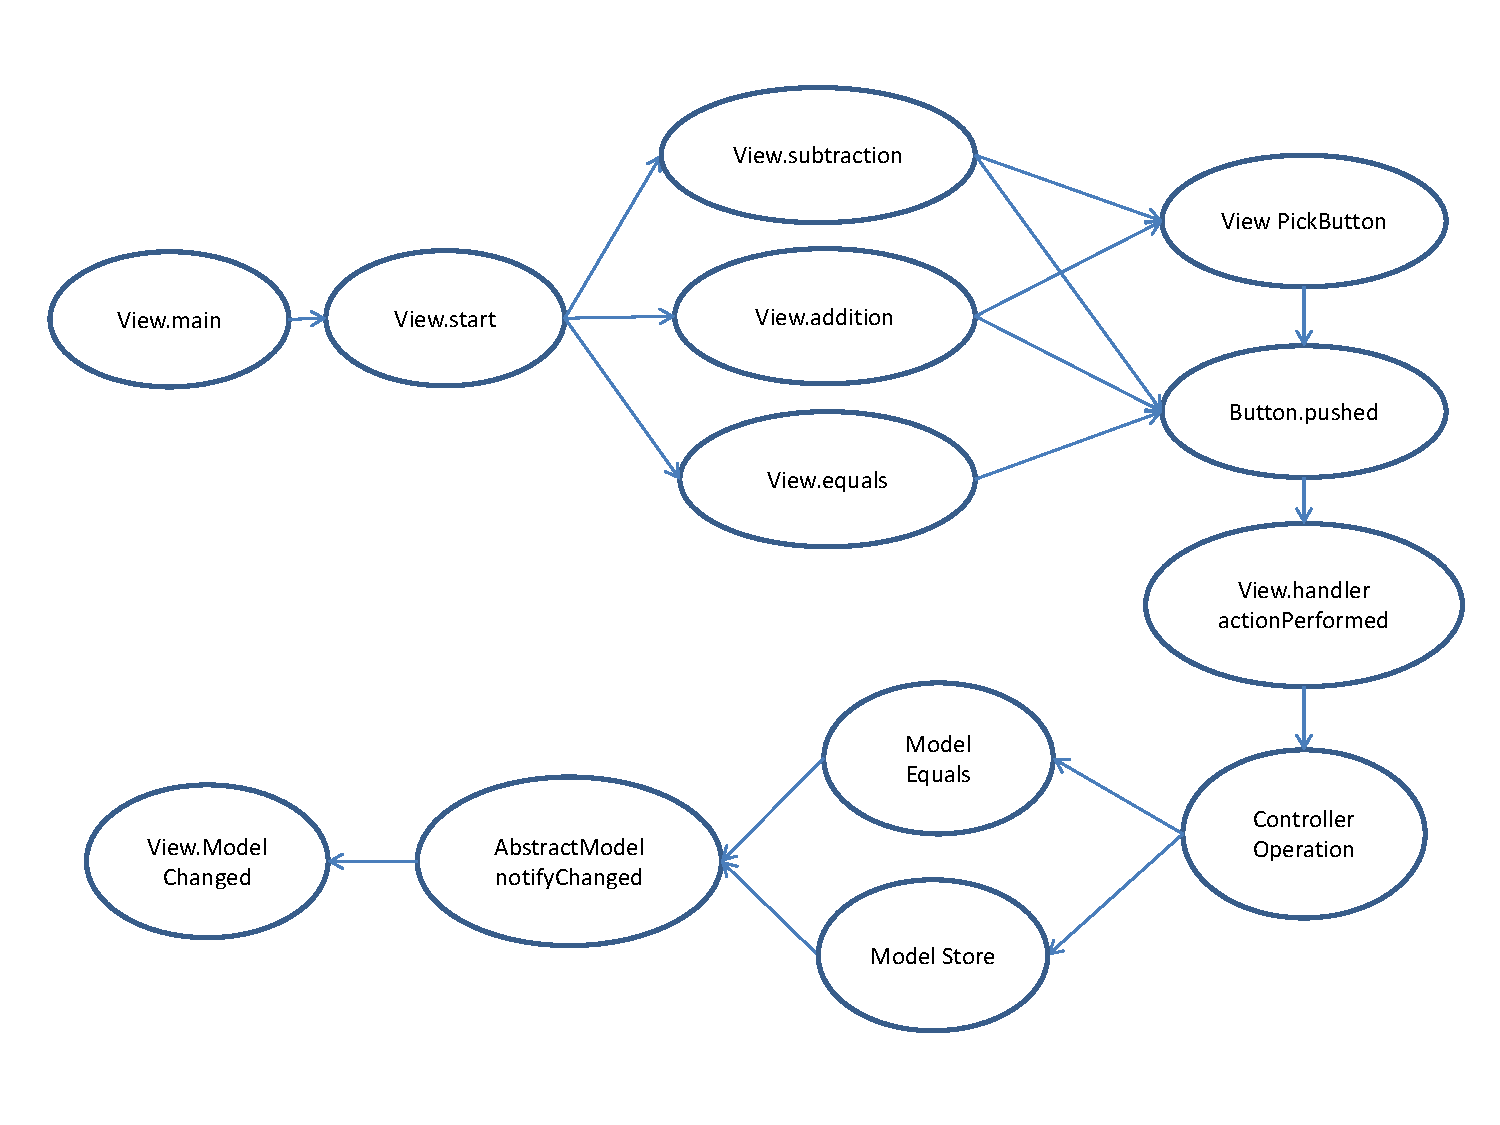
\includegraphics[keepaspectratio=true,scale=0.35]{noViolTrace.pdf}
  \caption{No violation case}
  \label{noViol}
\end{figure}

Figure~\ref{viol} shows the case with a violation. Method {\it actionPerformed} bypassed the {\it operation} method of Controller class and called a method from the Model directly. Because invocation of the {\it operation} method of Controller class was bypassed there was a violation. The transition in the call graph due to a violation is highlighted in red in Figure~\ref{viol}.

\begin{figure}
  \centering
  % Requires \usepackage{graphicx}
  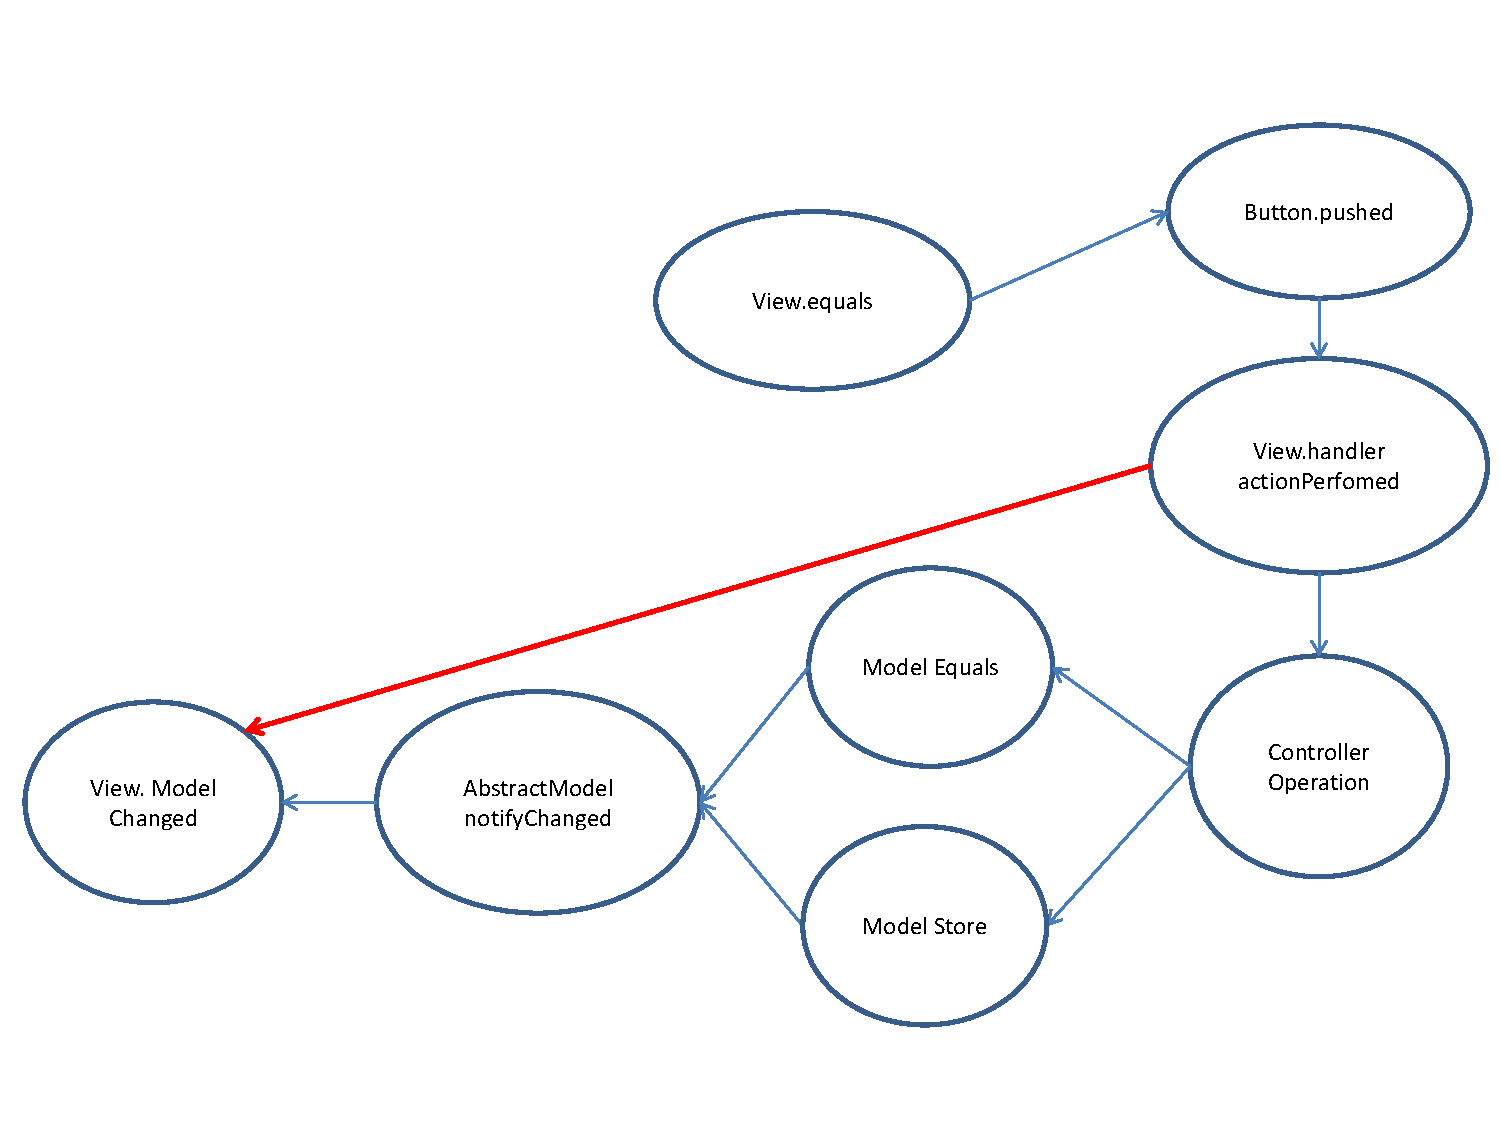
\includegraphics[keepaspectratio=true,scale=0.35]{violTrace.pdf}
  \caption{A case with a violation}
  \label{viol}
\end{figure}

Two cases were submitted to the analysis: a version with a violation of the constraint on sequence of method invocation and a version without a violation. In both cases there were multiple call graph paths from a given {\it pushed} method to a relevant method in the CalculatorModel class.

We show the paths found by the tool via manually created visualizations of transition graphs. They were created based on the output of SPF enhanced with the prototype implementation.

%\begin{figure}
%\begin{lstlisting}
%( calc.view.CalculatorView.modelChanged(Lcalc/model/ModelEvent;)V | (1368) Dist 3 )
%( calc.controller.CalculatorController.operation(Ljava/lang/String;)V | (1226) Dist 3 )
%( calc.model.CalculatorModel.store(I)V | (1262) Dist 4 )
%( calc.model.CalculatorModel.equals()V | (1658) Dist 4 )
%( calc.model.AbstractModel.notifyChanged(Lcalc/model/ModelEvent;)V | (1286) Dist 5 )
%\end{lstlisting}
%\caption{\label{alg:output}Sample of output}
%\end{figure}

%\begin{figure}
%\begin{lstlisting}
%elapsed time:       00:00:02
%states:             new=7,visited=14,backtracked=21,end=16
%search:             maxDepth=3,constraints=0
%choice generators:  thread=1 (signal=0,lock=1,sharedRef=0,threadApi=0,reschedule=0), data=5
%heap:               new=3843,released=1642,maxLive=500,gcCycles=17
%instructions:       25353
%max memory:         60MB
%loaded code:        classes=90,methods=1675
%\end{lstlisting}
%\caption{\label{alg:resNoViol}No violation result}
%\end{figure}

Figure~\ref{noViol} shows the case without a violation. In this case there was no path from the initial to the final method that violated the sequence constraint. All paths between the initial and final methods had an invocation of {\it operation} method of Controller class before the invocation of a relevant method in the CalculatorModel class.
The use of the call graph reduction algorithm reduced the initial call graph from 120 nodes in the whole call graph to 13 nodes encountered all the paths between the initial and final methods.


\section{Conclusion}
\label{sec:conclusion}

In this paper we described preliminary work focused on checking architectural constraints on sequences of method invocations. We gave a brief description of the prototype and a case study.
In the future we intend to add a general specification of the constraints via an appropriate logic and a testcase generation capability.
We also would like to perform a quantitative comparative analysis against similar approaches and improve the efficiency of the analysis algorithms.
In addition, we would like to validate the prototype by applying it to analysis of larger systems.


%ACKNOWLEDGMENTS are optional
% \section{Acknowledgments}

%
% The following two commands are all you need in the
% initial runs of your .tex file to
% produce the bibliography for the citations in your paper.
\bibliographystyle{abbrv}
\bibliography{rodion}
% \appendix

\balancecolumns
% That's all folks!
\end{document}
